%% ------------------------------------------------------------------------- %%
\chapter{Resultados}
\label{cap:resultados}

Neste capítulo apresentamos os resultados da avaliação do uso das redes convolucionais no problema de \textit{code retrieval}. Utilizamos a nossa arquitetura proposta no Capítulo~\ref{cap:abordagem}. E para comparar, utilizamos duas arquiteturas: uma arquitetura de referência \textit{Embedding} e outra arquitetura que é o estado da arte em recuperação de trecho de código-fonte proposta por \cite{cambronero-deep-learning-code-search:2019}. Os resultados da arquitetura CNN foram promissores. A arquitetura apresentou um valor de métrica \acrfull{mrr} de $0,70$. Em $75\%$ das vezes, as respostas corretas apareceram entre as 3 primeiras posições, de um total de 50 possíveis respostas. \todo{atualizar o valor}

\section{Avaliação}

Os resultados foram coletados a partir da avaliação dos modelos na amostra \emph{EVAL}. O valor final MRR é a média obtida após 20 iterações. Conforme a Tabela~\ref{table:resultados},  a arquitetura CNN obteve um resultado próximo da arquitetura bi-LSTM com CNN. Apesar do resultado ser relativamente menor, o seu tempo de duração de treinamento é de apenas 6s, enquanto o treinamento do bi-LSTM durou cerca de 48 minutos. Tanto o treinamento quanto a avaliação foram executadas na plataforma \Gls{colab} do Google. No momento de treinamento e coleta dos resultados, a execução foi feita em uma máquina virtual com acesso a uma \acrshort{vgpu} Tesla K80.

\begin{table}[H]
\centering
\begin{tabular}{ p{7cm} P{4cm} P{4cm} }
 \hline
    & \multicolumn{2}{c}{\textbf{Resultados}}\\
 \hline
 \textbf{Modelos} & \textbf{MRR} & \textbf{TOP1}\\
 \hline
 Embedding (m = $0.1$) & $0.637$& $0.493 \pm 0.009$\\
 
 Unif (m = $0.2$) & $0.675 \pm 0.006$ & $0.539 \pm 0.009$\\
 
 CNN / F = 1000 & $0.669 \pm 0.006$ & $0.527 \pm 0.012$\\
 
 CNN / F = 2000 & $0.673 \pm 0.007$ & $0.531 \pm 0.012$\\
 
 CNN / F = 4000 & $0.687 \pm 0.006$ & $0.553 \pm 0.011$\\
 
 CNN Compartilhado / F = 1000 & $0.678 \pm 0.007$ & $0.548 \pm 0.012$\\
 
 CNN Compartilhado / F = 2000 & $0.694 \pm 0.008$ & $0.565 \pm 0.012$\\
 
 CNN Compartilhado / F = 4000 & $0.700 \pm 0.004$ & $0.569 \pm 0.009$\\
 
 
 
 \hline
 
 Unif (m = $0.05$) com NL & $0.653 \pm 0.006$ & $0.515 \pm 0.011$\\
 
 CNN com NL / F = 1000 & $0.682 \pm 0.007$ & $0.543 \pm 0.012$\\
 
 CNN com NL / F = 2000 & $0.689 \pm 0.006$ & $0.553 \pm 0.011$\\
 
 CNN com NL / F = 4000 & $0.688 \pm 0.006$ & $0.553 \pm 0.011$\\
 
 \rowcolor{blue!40}
 CNN Compartilhado com NL / F = 1000 & $0.690 \pm 0.008$ & $0.553 \pm 0.015$\\
 
 CNN Compartilhado com NL / F = 2000 & $0.700 \pm 0.007$ & $0.573 \pm 0.012$\\
 
 CNN Compartilhado com NL / F = 4000 & $0.701 \pm 0.008$ & $0.577 \pm 0.015$\\
 
\hline
\end{tabular}
\caption{Resultado do modelo CNN em comparação com as outras arquiteturas \Gls{unif} e Embedding. MRR refere-se ao cálculo do Mean Reciprocal Rank da equação~\ref{eq:mrr}.}
\label{table:resultados}
\end{table}

Para entender um pouco melhor o resultado da média harmônica MRR, a figura abaixo exibe as posições da primeira ocorrência do trecho de código-fonte encontradas durante a avaliação dos modelos.

\begin{figure}[h]
    \centering
    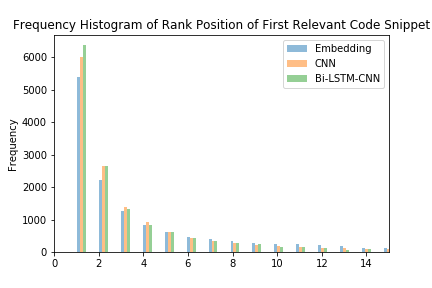
\includegraphics[width=1\textwidth]{figuras/cap-resultados-preliminares/histogram_results.png}
    \caption{Figura das primeiras posições observadas para o trecho de código-fonte anotado como correto.}
    \label{fig:histogram-mrr}
\end{figure}


Tanto o CNN quanto o bi-LSTM com CNN conseguiram classificar os trechos de código-fonte entre as 3 (três) primeiras posições em 75\% dos casos. O modelo bi-LSTM com CNN obteve uma precisão TOP-1 de 51\%, i.e., em mais da metade das vezes, o trecho de código-fonte relevante ficou na primeira posição. Já a nossa arquitetura proposta obteve um TOP-1 de aproximadamente 41\%. Um ponto a ser levantado é que a nossa métrica MRR só leva em consideração a posição apontada pelo modelo para o trecho de código-fonte anotado como correto. Mesmo que o modelo apresente um outro trecho de código-fonte que também é solução, o nosso método de avaliação não leva em consideração. Neste caso, o modelo é penalizado.

No exemplo a seguir\footnote{Este exemplo refere-se a questão \url{https://stackoverflow.com/questions/24593478/python-and-appending-items-to-text-and-excel-file}\label{foot:exemplo-resultados-preliminares}}, a rede bi-LSTM com CNN conseguiu apontar corretamente o trecho de código-fonte anotado como correto na primeira posição.
A nossa arquitetura CNN, apesar de não apresentar o trecho propriamente anotado, ele apresentou outro trecho que também serve como solução. Neste caso, apesar de ter sido penalizado, ele conseguiu responder a questão. Este é um ponto importante que teremos que analisar com cautela ao longo deste trabalho. 

\begin{tcolorbox}[colframe=orange!75!black,colback=gray!15!white,fonttitle=\bfseries,adjusted title=\large{Python and appending items to text and \colorbox{green}{excel} \colorbox{green}{file}}~\ref{foot:exemplo-resultados-preliminares},
enlarge top by=1cm%equivalent to mdframed 'skipabove'
]
\begin{mypython-without-margin}{bi-LSTM com CNN}
Yvalues = [1, 2, 3, 4, 5]
file_out = |\colorbox{green}{open}|('file.csv','wb')
mywriter=|\colorbox{green}{csv}|.|\colorbox{green}{writer}|(file_out, delimiter = '\n')
mywriter.|\colorbox{green}{writerow}|(Yvalues)
file_out.close()
\end{mypython-without-margin}

\begin{mypython-without-margin}{CNN}
import csv

with |\colorbox{green}{open}|("output.csv", "wb") as f:
    writer = |\colorbox{green}{csv}|.|\colorbox{green}{writer}|(f)
    writer.|\colorbox{green}{writerows}|(a)
\end{mypython-without-margin}

\end{tcolorbox}

\subsection{Ameaças à validade}

Conforme citado anteriormente, \cite{yao-2018} anotaram o conjunto de dados utilizando um framework proposto em seu artigo. Para anotá-los, os autores treinaram uma rede neural no conjunto de dados anotado manualmente. Em nosso trabalho, fizemos o caminho inverso. Treinamos os nossos modelos nos dados anotados automaticamente e avaliamos no conjunto anotado manualmente. Para diminuir o viés, adotamos o procedimento proposto por \cite{iyer-etal-2016-summarizing} descrito na Seções~\ref{sec:treinamento} e \ref{sec:avaliacao}.

\subsection{Considerações}

Os resultados apresentados pelo nosso modelo CNN parecem bastante promissores, a nosso ver. O próximo passo é comparar o nosso modelo com o modelo proposto por \cite{cambronero-deep-learning-code-search:2019}, que é o estado da arte. 

Não fizemos ajustes dos hiper-parâmetros e nem uso de regularização durante o treinamento. Na Figura \ref{fig:grafico-erro-cnn} abaixo, podemos ver que o CNN apresenta uma diferença grande entre a curva de erro na amostra de validação e da amostra de treinamento, principalmente a partir da época $5$ (eixo $X$), próximo da interrupção do treinamento. Isto é um indicativo de \textit{overfitting}. A arquitetura bi-LSTM com CNN apresenta o mesmo problema (ver Figura~\ref{fig:grafico-erro-bi-lstm-cnn}). Já no caso da arquitetura \textit{Embedding}, Figura \ref{fig:grafico-embedding}, as duas curvas de erro estão próximas até a interrupção. 

\begin{figure}[h]
    \centering
    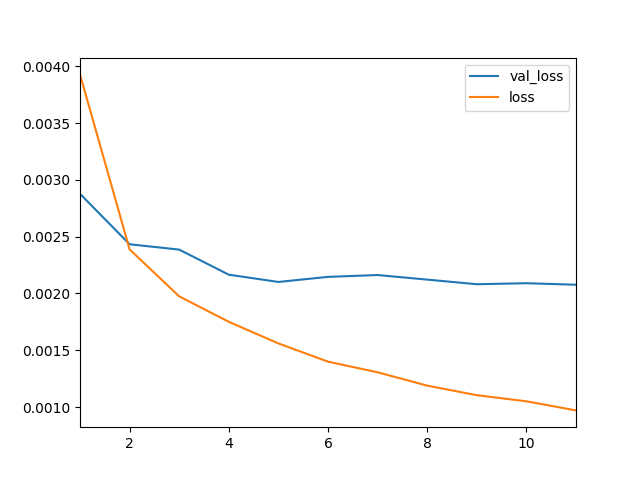
\includegraphics[width=1\textwidth]{figuras/cap-resultados-preliminares/569229_ConvolutionalLSTM_plot.png}
    \caption{Gráfico do treinamento do modelo bi-LSTM com CNN. Gráfico do erro de validação (\emph{val\_loss}) e erro na amostra de treinamento (\emph{loss}) por época (\emph{eixo X}). O melhor modelo em relação a métrica MRR foi obtido na época $9$.}
    \label{fig:grafico-erro-bi-lstm-cnn}
\end{figure}

\begin{figure}[h]
    \centering
    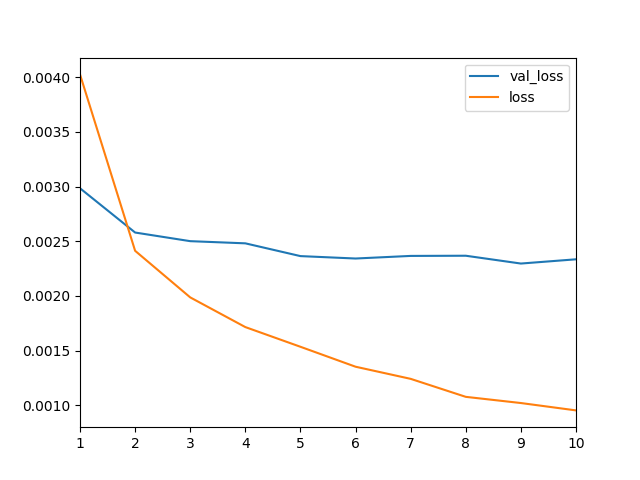
\includegraphics[width=1\textwidth]{figuras/cap-resultados-preliminares/569229_ConvolutionModel_plot.png}
    \caption{Gráfico do treinamento do CNN. Gráfico do erro de validação (\emph{val\_loss}) e erro na amostra de treinamento (\emph{loss}) por época (\emph{eixo X}). O melhor modelo em relação a métrica MRR foi obtido na época $9$.}
    \label{fig:grafico-erro-cnn}
\end{figure}

\begin{figure}[h]
    \centering
    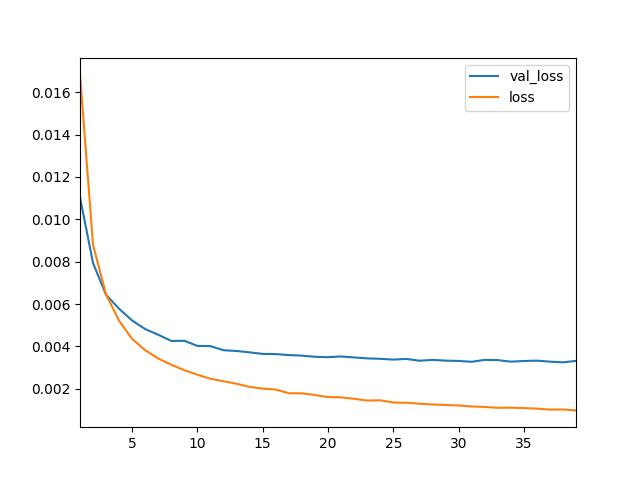
\includegraphics[width=1\textwidth]{figuras/cap-resultados-preliminares/569229_EmbeddingModel_plot.png}
    \caption{Gráfico do treinamento do modelo \textit{Embedding}. Gráfico do erro de validação (\emph{val\_loss}) e erro na amostra de treinamento (\emph{loss}) por época (\emph{eixo X}). O melhor modelo em relação a métrica MRR foi obtido na época $39$.}
    \label{fig:grafico-embedding}
\end{figure}

Podemos perceber que de acordo com as figuras~\ref{fig:grafico-erro-cnn} e \ref{fig:grafico-erro-bi-lstm-cnn}, tanto o CNN quanto o bi-LSTM com CNN tem uma margem a melhorar. Além da margem de melhora no treinamento, uma análise mais detalhada do resultado é necessária. Conforme o exemplo citado na seção anterior, o modelo CNN apresentou uma resposta correta para a pergunta, porém foi penalizada pois não era exatamente o trecho anotado como correto. Caso haja mais casos deste tipo, podemos adotar o mesmo procedimento proposto por \cite{cambronero-deep-learning-code-search:2019} de avaliação automática. Um trecho será considerado correto quando a diferença do resultado da função $h_{\theta}$ de similaridade entre ele e o trecho anotado como correto estiver dentro de um certo intervalo.
